\section{Fingerprint Localization}
\label{sec:localization}

This section applies the fingerprint matrix obtained from the ray-tracing
dataset (Section~\ref{sec:dataset}) to the user-positioning task.
Each row of the matrix corresponds to one UE grid position and encodes a
CSI-derived feature vector of dimension $D_f = 3690$ drawn from the nine
BS sites; the associated label is the UE 2-D ground-truth coordinate
$(x,y)$.
Out of the $N=3\,186$ valid grid points, 70\% (2\,230) are used for
training and 30\% (956) for testing, with the split drawn uniformly at
random.

Six methods are evaluated, grouped into a non-parametric baseline and a
set of neural estimators~\cite{hoydis2023sionna_rt,3gpp_nr_channel}:
\begin{itemize}
  \item \textbf{wKNN (IDW)}: inverse-distance-weighted $k$-nearest
        neighbours with $k=3$ and Minkowski exponent $p=3$.  Each test
        point is estimated as the IDW-weighted centroid of its nearest
        fingerprints in the library.
  \item \textbf{wKNN Coarse-to-Fine (C2F)}: $k=9$, $p=3$, radius
        $R=5\,\text{m}$.  Coarse candidates are filtered spatially
        before the IDW weighting, with a fall-back to plain wKNN when
        the radius contains too few candidates.
  \item \textbf{NN Regression}: a fully-connected multilayer perceptron
        (MLP) that regresses the 2-D UE coordinates directly from the
        flat fingerprint vector, trained with a Huber loss.
  \item \textbf{NN Classification}: an MLP that maps each fingerprint to
        one of the discrete $2.5\,\text{m}$ grid cells.
  \item \textbf{CNN Regression}: a 1-D/2-D convolutional regressor that
        reshapes the fingerprint into a $(410 \text{ feat}/\text{TX})
        \times 9\,\text{TX}$ image and applies cross-BS
        convolutions.
  \item \textbf{Ensemble}: an average of five independently-initialised
        MLP regressors.
\end{itemize}

Following two methods were implemented using matlab:
\begin{itemize}
 \item \textbf{wKNN}: inverse-distance-weighted $k$-nearest
        neighbours with $k=1,3, 5, 7, 9, 11$ where closer neighbors have more influence 
        on the final estimation and all features are considered uniformly. 
        $k=9$ was found to be the best performing value.  
\item \textbf{NN Regression, MLP)}: Standard fully-connected Multilayer Perceptron (MLP) 
for regression predicting continuous coordinates. The NN had 4 hidden layers with  
256, 128, 64, and 2 neurons respectively. The ReLU activation function was used 
for the hidden layers and the output layer had a linear activation function. 
The model was trained using the Adam optimizer with initial learning rate: 0.0005. At every 400 epochs the learning rate 
 was halved. 

\end{itemize}


\subsection{Performance Metrics}

Per-sample localization error is defined as the Euclidean distance
between the estimate and the ground-truth 2-D coordinate:
\begin{equation}
  e_n = \bigl\lVert \hat{\mathbf{p}}_n - \mathbf{p}_n \bigr\rVert_2,
  \qquad n = 1,\dots,N_{\mathrm{test}}.
\end{equation}
From this sequence we compute the mean absolute error (MAE), the
root-mean-square error (RMSE), the median, and the 90\,\% / 95\,\%
percentiles of the error CDF.

\subsection{Results}

Table~\ref{tab:loc_results} summarises the test-set performance on the
Otaniemi\_small scene. Fig.~\ref{fig:loc_cdf}  shows the empirical
error CDFs. Fig.~\ref{fig:loc_matcdf} shows CDF of the matlab wKNN 
and Fig.~\ref{fig:loc_matwknnheat} shows the corresponding heatmap.  



\begin{table}[htbp]
\caption{Fingerprint-localization test performance on Otaniemi\_small
         ($N_{\mathrm{test}} = 956$)}
\label{tab:loc_results}
\centering
\resizebox{\columnwidth}{!}{%
\begin{tabular}{lrrrrr}
\toprule
Method & MAE (m) & RMSE (m) & Median (m) & P90 (m) & P95 (m) \\
\midrule
wKNN (IDW)          & 13.74 & 21.04 & 7.98  & 33.38  & 45.12  \\
wKNN C2F            & 13.77 & 21.07 & 8.01  & 33.41  & 45.94  \\
wKNN (matlab IDW)   & 18.24 & 27.25 & 10.14 & 4608  &  -  \\
NN Regression       &  9.53 & 12.34 & 7.90  & 17.11  & 20.75  \\
NN (MLP matlab)     & 16.31 & 24.27 & 10.24 & 37.40  & -  \\
NN Classification   & 68.32 & 78.10 & 62.52 & 122.75 & 134.68 \\
CNN Regression      & 10.56 & 14.21 & 7.85  & 20.30  & 28.49  \\
Ensemble (5 MLPs)   & 10.29 & 13.65 & 8.00  & 19.90  & 27.03  \\
\bottomrule
\end{tabular}%
}
\end{table}

\begin{figure}[htbp]
  \centering
  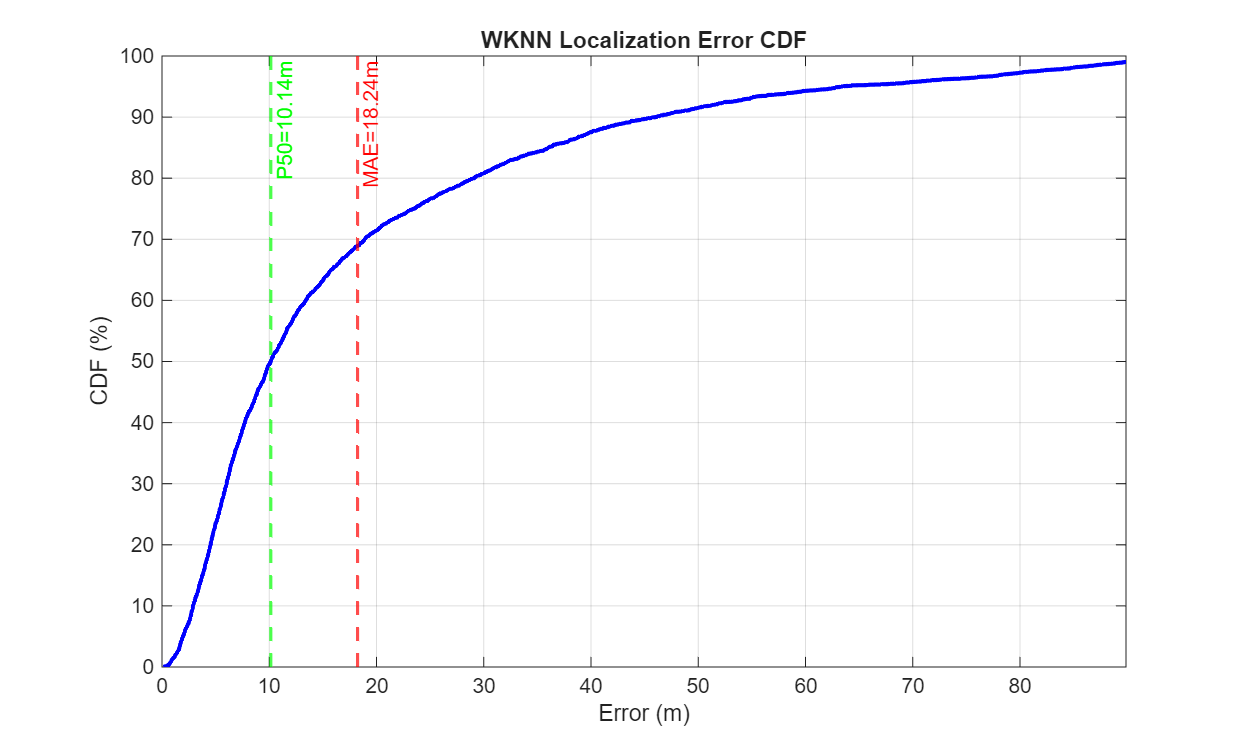
\includegraphics[width=\columnwidth]{pictures/03_localization/wknn_cdf_1.png}
  \caption{Empirical CDF of localization error for the matlab wKNN method.}
  \label{fig:loc_matcdf}
\end{figure}

\begin{figure}[htbp]
  \centering
  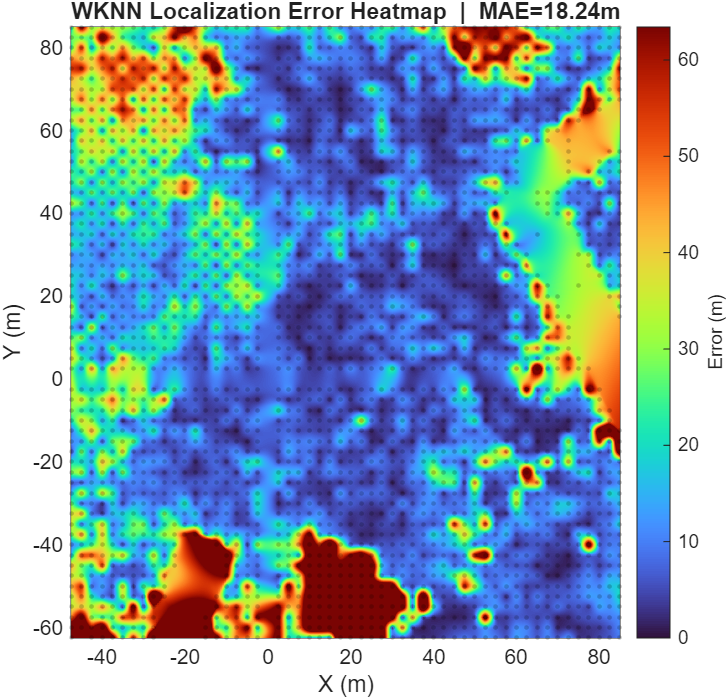
\includegraphics[width=\columnwidth]{pictures/03_localization/wknn_error_heatmap.png}
  \caption{Heatmap of localization error for the matlab wKNN method.}
  \label{fig:loc_matwknnheat}
\end{figure}

\begin{figure}[htbp]
  \centering
  
\includegraphics[width=\columnwidth]{pictures/03_localization/localization_error_cdf.png}
  \caption{Empirical CDF of test-set localization error for the six
           evaluated methods.  A curve shifted towards the left
           indicates better performance for a given error budget.}
  \label{fig:loc_cdf}
\end{figure}


\begin{figure}[htbp]
  \centering
  
\includegraphics[width=\columnwidth]{pictures/03_localization/localization_metrics_comparison.png}
  \caption{Metric-by-metric comparison of the six localizers
           (MAE, RMSE, median, P90, P95).}
  \label{fig:loc_metrics}
\end{figure}

\begin{figure*}[htbp]
  \centering
  
\includegraphics[width=\textwidth]{pictures/03_localization/localization_error_heatmaps.png}
  \caption{Spatial test-set error heatmaps for each method.  Colours
           indicate the Euclidean localization error at each UE
           position; grey cells correspond to grid points reserved for
           training.}
  \label{fig:loc_heatmaps}
\end{figure*}

The NN regressor is the clear winner ($\text{MAE}=9.53\,\text{m}$,
$\text{RMSE}=12.34\,\text{m}$) and its CDF dominates all competitors
above the $P_{85}$ level.
The ensemble of five MLPs reaches a similar median error but slightly
lower tail robustness.
Both wKNN variants and the CNN regressor cluster around $10$--$14\,\text{m}$
MAE, illustrating that the fingerprint vector already contains enough
cross-BS information to make simple nearest-neighbour matching
competitive with a vanilla CNN.
The NN classifier, by contrast, fails almost completely
($\text{MAE}\approx 68\,\text{m}$, $0\,\%$ exact-cell accuracy):
with 3\,186 grid cells and only 2\,230 training rows there is on average
less than one labelled fingerprint per class, so the classification head
cannot separate adjacent cells.

Training curves for the NN and CNN regressors are shown in
Figs.~\ref{fig:nn_train} and~\ref{fig:cnn_train}; both networks converge
smoothly without obvious over-fitting.

\begin{figure}[htbp]
  \centering
  
\includegraphics[width=\columnwidth]{pictures/03_localization/nn_regression_training.png}
  \caption{NN-regression training curve on the Otaniemi\_small fingerprint
           dataset (Huber loss vs.\ epoch, train/val).}
  \label{fig:nn_train}
\end{figure}

\begin{figure}[htbp]
  \centering
  
\includegraphics[width=\columnwidth]{pictures/03_localization/cnn_regression_training.png}
  \caption{CNN-regression training curve (Huber loss vs.\ epoch,
           train/val).}
  \label{fig:cnn_train}
\end{figure}

\subsection{Discussion}

The dominant error source is spatial ambiguity between geometrically
similar NLOS regions of the scene: parts of the grid that lie behind
large building facades produce very similar CSI vectors across all nine
BSs, which the learned regressor cannot disambiguate without additional
features.
Fig.~\ref{fig:loc_heatmaps} makes this visible --- the largest errors
cluster around shadow regions and along the corridors where none of the
nine BSs provides a strong LOS component.
The following practical levers would directly reduce the errors, in
order of expected impact:
\begin{itemize}
  \item \textbf{More BS diversity}: increasing the number of sites, or
        spacing the existing nine more evenly, would reduce the NLOS
        shadow regions and improve the conditioning of the fingerprint
        matrix~\cite{3gpp_nr_channel}.
  \item \textbf{Angular features}: adding the Sionna AoA/AoD angles
        (available in the Sionna dataset, Section~\ref{sec:dataset}) to the fingerprint would provide
        a direction-of-arrival cue that is complementary to the amplitude
        spectrum~\cite{hoydis2023sionna_rt}.
  \item \textbf{CNN architecture}: organising the fingerprint as a
        $(N_{\mathrm{BS}}\times N_{\mathrm{sc}})$ image with explicit
        cross-BS channels, plus per-BS batch normalisation, would let the
        CNN exploit the site geometry more effectively than the flat
        reshape used here.
  \item \textbf{Feature selection}: the ablation study in
        Section~\ref{sec:ablation} shows that dropping the raw OFDM taps
        and keeping only the 90-feature
        ``Light'' subset (TDoA+AoA+RSS+Rch) reduces MAE from
        $9.53\,\text{m}$ to $6.58\,\text{m}$ --- the single largest
        improvement observed on this dataset, and achieved with no
        architectural changes.
\end{itemize}

\subsection{Feature Ablation Study}
\label{sec:ablation}

To understand which CSI feature families actually drive the localization
performance, an ablation was run on the Otaniemi\_small dataset over 22
combinations of the eight candidate feature groups: raw OFDM taps,
time-difference-of-arrival (TDoA), angle-of-arrival (AoA), received
signal strength (RSS), path-loss (PL), per-path delay (Dly), covariance
eigenvalues (CovE), and a LOS-reached indicator (Rch).
For each combination the three regression heads from
Section~\ref{sec:localization} (wKNN, NN, CNN) were re-trained on an
identical train/test split and scored by MAE, RMSE and $P_{90}$.
Table~\ref{tab:ablation} lists the best MAE for each feature combination,
sorted from best to worst.

\begin{table}[htbp]
\caption{Feature-ablation results on Otaniemi\_small.  ``Best MAE'' is
         the minimum across the three regressors; ``Method'' names the
         winner.  Feature families: OFDM = raw OFDM taps,
         TDoA = time-difference of arrival, AoA = angle of arrival,
         RSS = received power, PL = path loss, Dly = per-path delay,
         CovE = covariance eigenvalues, Rch = reached/LOS flag.}
\label{tab:ablation}
\centering
\resizebox{\columnwidth}{!}{%
\begin{tabular}{lrlrl}
\toprule
Combination          & $N_{\mathrm{feat}}$ & Features                      & Best MAE (m) & Method \\
\midrule
Light                & 90                   & TDoA+AoA+RSS+Rch              & \textbf{6.58} & NN Reg \\
No\_OFDM\_Light      & 108                  & TDoA+AoA+RSS+PL+Dly+Rch       & 6.61          & CNN Reg \\
Solo\_AoA            & 36                   & AoA                           & 7.48          & CNN Reg \\
No\_OFDM             & 135                  & TDoA+AoA+RSS+PL+Dly+CovE+Rch  & 7.48          & CNN Reg \\
Geometry             & 81                   & TDoA+AoA+Dly                  & 7.60          & CNN Reg \\
Solo\_RSS            & 9                    & RSS                           & 9.94          & wKNN \\
Radio                & 27                   & RSS+PL+Rch                    & 10.61         & wKNN \\
No\_Reached          & 3681                 & OFDM+TDoA+AoA+RSS+PL+Dly+CovE & 9.47          & NN Reg \\
No\_TDoA             & 3654                 & OFDM+AoA+RSS+PL+Dly+CovE+Rch  & 9.64          & NN Reg \\
No\_Delay            & 3681                 & OFDM+TDoA+AoA+RSS+PL+CovE+Rch & 9.73          & NN Reg \\
No\_CovEig           & 3663                 & OFDM+TDoA+AoA+RSS+PL+Dly+Rch  & 9.83          & NN Reg \\
No\_RSS              & 3681                 & OFDM+TDoA+AoA+PL+Dly+CovE+Rch & 9.94          & NN Reg \\
No\_PathLoss         & 3681                 & OFDM+TDoA+AoA+RSS+Dly+CovE+Rch & 10.02        & NN Reg \\
No\_AoA              & 3654                 & OFDM+TDoA+RSS+PL+Dly+CovE+Rch & 13.34         & NN Reg \\
OFDM\_Radio          & 3573                 & OFDM+RSS+PL                   & 13.83         & NN Reg \\
Solo\_OFDM           & 3555                 & OFDM                          & 13.93         & NN Reg \\
Spectral             & 3555                 & OFDM                          & 14.09         & NN Reg \\
Solo\_CovEig         & 27                   & CovE                          & 32.45         & CNN Reg \\
Solo\_Reached        & 9                    & Rch                           & 50.78         & CNN Reg \\
Solo\_PathLoss       & 9                    & PL                            & 50.87         & CNN Reg \\
Solo\_Delay          & 9                    & Dly                           & 51.19         & CNN Reg \\
Solo\_TDoA           & 36                   & TDoA                          & 52.51         & NN Reg \\
\bottomrule
\end{tabular}%
}
\end{table}

Four observations are worth highlighting:

\paragraph{AoA dominates.}
The 36-feature \texttt{Solo\_AoA} configuration already reaches
$7.48\,\text{m}$ MAE, beating every combination that includes the full
3\,555 raw OFDM taps.  Angles of arrival across the nine BS sites carry
most of the useful geometric signal in a multi-BS outdoor
scene~\cite{3gpp_nr_channel}.

\paragraph{Raw OFDM hurts more than it helps.}
wKNN on \texttt{Solo\_OFDM} reaches only $15.01\,\text{m}$ MAE, roughly
double the compact combinations.  The 3\,555 frequency taps dominate the
Euclidean distance computation used by wKNN and obscure the geometric
features; the NN regressor can partially learn to filter them
(MAE $\sim 10\,\text{m}$) but the full-feature baseline still
\emph{loses} to the 90-feature \texttt{Light} set
($6.58\,\text{m}$) --- a textbook curse-of-dimensionality
effect~\cite{vandermaaten2008tsne}.

\paragraph{Single scalar features are useless alone but useful in combination.}
\texttt{Solo\_TDoA}, \texttt{Solo\_Delay}, \texttt{Solo\_PathLoss} and
\texttt{Solo\_Reached} all collapse to $50$--$56\,\text{m}$ MAE on their
own because each scalar is geometrically ambiguous across the scene.
Yet \emph{removing} any one of them from the full stack measurably
worsens the result (\emph{e.g.}\ removing AoA lifts wKNN from
$7.76$ to $14.82\,\text{m}$), showing that their value lies in the
joint manifold rather than in any individual coordinate.

\paragraph{Sweet spot: the Light configuration.}
The 90-feature \texttt{Light} set (TDoA+AoA+RSS+Rch) attains the best
overall MAE ($6.58\,\text{m}$, NN regression), a 31\,\% improvement on
the 3\,690-feature baseline used in Section~\ref{sec:localization}
($9.53\,\text{m}$), with $97.6\,\%$ fewer features and correspondingly
faster training and inference.
This set is therefore the recommended working point for any follow-on
Otaniemi experiments and is consistent with the feature guidance in the
broader channel-charting literature~\cite{studer2018channel_charting}.


\subsection{MATLAB Pipeline Cross-Check in Python environment}
\label{sec:matlab_localization}

As an independent sanity check the same six localizers were re-run on the
MATLAB-derived amd introduced in
Section~\ref{sec:matlab_dataset}.
The MATLAB fingerprints use only four feature families
(AoA+RSS+Dly+Rch, $D_f = 63$) and are built by the scripts in
\texttt{hannunfilet/}: \texttt{otavectorizedv3.m} (ray tracing on the
OSM model), \texttt{build\_fingerprint\_db\_v3.m} (feature assembly),
\texttt{finger\_WKK.m} (wKNN with a $k$ sweep and leave-one-out CV),
\texttt{mpl\_localization.m} (MLP regression), and
\texttt{cnn1d\_localization.m} (1-D CNN regression).
The $N = 3\,069$ UEs are split 70/30 using the same random seed as the
Sionna pipeline, giving $N_{\mathrm{test}} = 921$.
Table~\ref{tab:loc_matlab} lists the corresponding test-set metrics.

\begin{table}[htbp]
\caption{Fingerprint-localization test performance on the MATLAB ($N_{\mathrm{test}} = 921$, $D_f = 63$).}
\label{tab:loc_matlab}
\centering
\resizebox{\columnwidth}{!}{%
\begin{tabular}{lrrrrr}
\toprule
Method & MAE (m) & RMSE (m) & Median (m) & P90 (m) & P95 (m) \\
\midrule
wKNN (IDW)        & 18.29 & 29.88 &  7.58 &  57.57 &  75.18 \\
wKNN C2F          & 18.18 & 30.05 &  7.16 &  57.23 &  75.35 \\
NN Regression     & 19.79 & 29.03 & 11.06 &  54.70 &  71.93 \\
NN Classification & 69.30 & 78.82 & 64.90 & 125.02 & 135.37 \\
CNN Regression    & 20.40 & 28.94 & 12.51 &  54.06 &  71.37 \\
Ensemble (5 MLPs) & 18.38 & 27.85 &  9.64 &  55.09 &  68.40 \\
\bottomrule
\end{tabular}%
}
\end{table}

Compared to the Sionna corpus (Table~\ref{tab:loc_results}), the MATLAB
corpus is roughly $2\times$ harder: the best MAE rises from
$9.53\,\text{m}$ to $18.18\,\text{m}$ and the $P_{90}$ tail grows
substantially.
Two effects drive this gap: (i)~the MATLAB feature vector has only 63
columns against 3\,690, so there is less redundancy available to the
learner; and (ii)~the MATLAB ray tracer produces a sparser set of
recovered paths in the deep-NLOS corners of the scene, consistent with
the geometric-only reflection model of the MATLAB RT toolbox.
The classifier head again collapses for the same reason as in the
Sionna case: 3\,069 fine-grained grid cells with only $\sim\!2\,148$
training samples.


